\documentclass{beamer}
%\documentclass[handout]{beamer}

% This file is a solution template for:

% - Giving a talk on some subject.
% - The talk is between 15min and 45min long.
% - Style is ornate.

% Copyright 2004 by Till Tantau <tantau@users.sourceforge.net>.
%
% In principle, this file can be redistributed and/or modified under
% the terms of the GNU Public License, version 2.
%
% However, this file is supposed to be a template to be modified
% for your own needs. For this reason, if you use this file as a
% template and not specifically distribute it as part of a another
% package/program, I grant the extra permission to freely copy and
% modify this file as you see fit and even to delete this copyright
% notice. 


\mode<presentation>
{
  \usetheme{Montpellier}

  %\setbeamercovered{transparent}
  % or whatever (possibly just delete it)
}

\usepackage{xmpmulti} % package that defines \multiinclude

\usepackage[english]{babel}

\usepackage[utf8]{inputenc}

%\usepackage[latin1]{inputenc}

\usepackage{times}
\usepackage[T1]{fontenc}
% Or whatever. Note that the encoding and the font should match. If T1
% does not look nice, try deleting the line with the fontenc.

\title[\ouralg] % (optional, use only with long paper titles)
{Exponential Weights Algorithms for Online Learning}

\author[Freund] % (optional, use only with lots of authors)
{Yoav Freund}
\date{}

% - Give the names in the same order as the appear in the paper.
% - Use the \inst{?} command only if the authors have different
%   affiliation.

\institute[Universities of Somewhere and Elsewhere] % (optional, but mostly needed)

\subject{Machine Learning}
% This is only inserted into the PDF information catalog. Can be left
% out. 

% If you have a file called "university-logo-filename.xxx", where xxx
% is a graphic format that can be processed by latex or pdflatex,
% resp., then you can add a logo as follows:

% \pgfdeclareimage[height=0.5cm]{university-logo}{university-logo-filename}
% \logo{\pgfuseimage{university-logo}}



% Delete this, if you do not want the table of contents to pop up at
% the beginning of each subsection:
%% \AtBeginSubsection[]
%% {
%%   \begin{frame}<beamer>
%%     \frametitle{Outline}
%%     \tableofcontents[currentsection,currentsubsection]
%%   \end{frame}
%% }


% If you wish to uncover everything in a step-wise fashion, uncomment
% the following command: 

\beamerdefaultoverlayspecification{<+->}

% \newcommand{\R}[1]{{\color{red}{#1}}}
% \newcommand{\W}{\vec{W}}
% \newcommand{\V}{\vec{V}}
% \newcommand{\X}{\vec{X}}
% \newcommand{\loss}{\vec{\ell}}
% \newcommand{\HedgeLoss}{L_{\mbox{\footnotesize Hedge}}}

\newcommand{\newmcommand}[2]{\newcommand{#1}{{\ifmmode {#2}\else\mbox{${#2}$}\fi}}}
\newcommand{\newmcommandi}[2]{\newcommand{#1}[1]{{\ifmmode {#2}\else\mbox{${#2}$}\fi}}}
\newcommand{\newmcommandii}[2]{\newcommand{#1}[2]{{\ifmmode {#2}\else\mbox{${#2}$}\fi}}}
\newcommand{\newmcommandiii}[2]{\newcommand{#1}[3]{{\ifmmode {#2}\else\mbox{${#2}$}\fi}}}

\newcommand{\algfnt}{\bf}

\newmcommand{\ouralg}{{\mbox{\algfnt Hedge}({\eta})}}

\newmcommand{\iter}{T}

\newfont{\cmmib}{cmmib10}
\newcommand{\boldell}{{\mbox{\cmmib \symbol{'140}}}}

\newmcommandi{\costvec}{{\boldell}^{#1}}
\newmcommandii{\cost}{{\ell}^{#1}_{#2}}

\newmcommandi{\rd}{\tilde{#1}}

\newmcommandi{\distvec}{{\bf p}^{#1}}
\newmcommandi{\rddistvec}{\rd{\bf p}^{#1}}
\newmcommandii{\dist}{{p}^{#1}_{#2}}
\newmcommandii{\rddist}{\rd{p}^{#1}_{#2}}

\newmcommandi{\bdistvec}{{\bf q}^{#1}}
\newmcommandii{\bdist}{{q}^{#1}_{#2}}

\newmcommandi{\wtvec}{{\bf w}^{#1}}
\newmcommandi{\rdwtvec}{\rd{\bf w}^{#1}}
\newmcommandii{\wt}{{w}^{#1}_{#2}}
\newmcommandii{\rdwt}{\rd{w}^{#1}_{#2}}

\newcommand{\w}[1]{\makebox[12pt]{{#1}}}
\newcommand{\Rps}{\mbox{\tt R}}
\newcommand{\rPs}{\mbox{\tt P}}
\newcommand{\rpS}{\mbox{\tt S}}
\newcommand{\rpstie}{\w{$\frac{1}{2}$}}
\newcommand{\rpswin}{\w{$0$}}
\newcommand{\rpsloss}{\w{$1$}}

\newmcommand{\decspace}{\Delta}
\newmcommand{\decsym}{\delta}
\newmcommandi{\dec}{\decsym^{#1}}
\newmcommand{\decdistsym}{\cal D}
\newmcommandi{\decdist}{{\decdistsym}^{#1}}

\newmcommand{\simpdistspace}{{\bf \cal S}}
\newmcommand{\domset}{{\rm dom}(\decdistsym)}

\newmcommand{\expdistsym}{{\cal E}}
\newmcommandii{\expdist}{{\expdistsym}^{#1}_{#2}}
\newmcommand{\expdecsym}{{\varepsilon}}
\newmcommandii{\expdec}{\expdecsym^{#1}_{#2}}

\newmcommand{\outspace}{\Omega}
\newmcommand{\outsym}{\omega}
\newmcommandi{\out}{\outsym^{#1}}

%\newmcommandii{\Dkl}{D_{\mbox{kl}}\paren{#1||#2}}
\newmcommandii{\Dkl}{{\rm {KL}}\paren{{#1}\;||\;{#2}}}

\newmcommandi{\sumwts}{\sum_{i=1}^N \wt{#1}{i}}

\newmcommand{\lossalg}{L_A}
\newmcommand{\lossouralg}{{L_{\mbox{\scriptsize\algfnt Hedge}(\eta)}}}
\newmcommand{\lossS}{{L_{\mbox{\scriptsize\algfnt S}}}}
\newmcommandi{\lossi}{L_{#1}}
\newmcommandii{\lossit}{L_{#1}^{#2}}

\newmcommandi{\upbnd}{\tilde{#1}}

\newcommand{\angles}[1]{{\left\langle {#1} \right\rangle}}
\newcommand{\paren}[1]{{\left( {#1} \right)}}
\newcommand{\abs}[1]{{\left| {#1} \right|}}
\newcommand{\ceiling}[1]{{\left\lceil {#1} \right\rceil}}

\newfont{\msym}{msbm10}
\newcommand{\real}{\mbox{\msym R}}

\newmcommand{\updatefcn}{U_\eta}

%% \newtheorem{theorem}{Theorem}	
%% \newtheorem{lemma}[theorem]{Lemma}
%% \newtheorem{corollary}[theorem]{Corollary}
%% \newtheorem{definition}{Definition}

%\newcommand{\proof}{\noindent{\bf Proof:} }
%\newcommand{\example}[1]{{\em Example #1.} }
%\newcommand{\qed}{\rule{0.7em}{0.7em}}

\newcommand{\WeakAlg}{\mbox{\algfnt WeakLearn}}
\newcommand{\Boost}{\mbox{\algfnt AdaBoost}}
\newcommand{\EX}{\mbox{\bf EX}}
\newmcommand{\hf}{h_{{f}}}
\newmcommand{\rdhf}{\rd{h}_{{f}}}
\newmcommand{\hfT}{h^T_{{f}}}
\newmcommand{\ranh}{{b}}

\newmcommand{\conclass}{{\cal C}}

\newmcommand{\badvec}{{\bf b}}
\newmcommandi{\bad}{{b}_{#1}}

%%%%%%%% New commands defined for the game-playing paper

\newmcommand{\hedge}{\algfnt Hedge}
\newmcommand{\play}{\algfnt Play}
\newmcommandi{\Glossvec}{{\bg y}^{#1}}
\newmcommandii{\Gloss}{{y}^{#1}_{#2}}
%\newmcommandi{\action}{{I}_{#1}}
\newmcommandi{\Gdistvec}{{\bf \tilde{p}}^{#1}}
\newmcommandii{\Gdist}{{\teilde{p}}^{#1}_{#2}}

%%%%%%%%%%%%%%%%%%%%%%%%%%%%%%%%%%%%%%%%%%%%%%%%%%%%%
\newmcommand{\Idistvec}{{D}}
\newmcommandi{\Idist}{\Idistvec({#1})}
\newmcommand{\Idistt}{\Idistvec_t}

\newmcommand{\Xdist}{{\cal P}}
\newmcommand{\emp}{\hat{\epsilon}}

\newmcommand{\classpc}{Y}
\newmcommand{\numclass}{k}
\newmcommandii{\prob}{\mbox{\rm Pr}_{#1}\left[{#2}\right]}
\newmcommandii{\exval}{\mbox{\rm E}_{#1}\left[{#2}\right]}

\newmcommand{\lab}{y}
\newmcommand{\ploss}{\mbox{ploss}}
\newmcommandii{\avploss}{\ploss_{#1}({#2})}
\newcommand{\sfrac}[2]{\mbox{$\frac{#1}{#2}$}}

\newcommand{\mboosta}{\mbox{\algfnt AdaBoost.M1}}
\newcommand{\mboostb}{\mbox{\algfnt AdaBoost.M2}}
\newcommand{\mboostr}{\mbox{\algfnt AdaBoost.R}}

\newmcommand{\slos}{\mbox{ploss}}
\newmcommandiii{\sloss}{\slos_{#1}({#2},{#3})}
\newmcommandiii{\avsloss}{\slos_{{#1},{#2}}({#3})}

\newmcommandii{\vwt}{{W}^{#1}_{#2}}

\newcommand{\figline}{\rule{\textwidth}{1pt}}

%\newmcommandi{\1}{{\bf 1}({#1})}
\newmcommandi{\1}{[\![{#1}]\!]}

\newmcommand{\confcn}{\kappa}
\newmcommandi{\erint}{\abs{\int_{y_i}^{h_t(x_i)} {#1} dy}}
%\newmcommandi{\erint}{\int_{\min\{y_i,h_t(x_i)\}}^{\max\{y_i,h_t(x_i)\}}{#1}dy}


\begin{document}

\begin{frame}
  \titlepage
  \begin{small}
  \end{small}
\end{frame}


\begin{frame}{Probably Approximately Correct (PAC) Learning}
  \begin{itemize}
    \item Sample space \R{$X$} with a fixed but unknown distribution \R{$P$}.
    \item Concept class \R{$C$}, with \R{$c \in C$} and \R{$c : X \to \{0,1\}$}.
    \item \textbf{Learning Input}: A training set \R{$\{(x_1,y_1), \ldots, (x_n,y_n)\}$} 
          drawn i.i.d.\ according to \R{$P$}, labeled by some \R{$c \in C$}.
    \item \textbf{Learning Output}: A concept \R{$c'$} such that 
      \[
         \R{P\bigl(c(x) \neq c'(x)\bigr) \leq \epsilon}
      \]
    \item \textbf{Strong PAC Learning} of \R{$C$}: There exists an algorithm such that 
      for all \R{$\epsilon$}, \R{$\delta$}, the algorithm runs in time polynomial 
      in \R{$1/\epsilon$} and \R{$1/\delta$} and outputs \R{$c'$} with
      \[
        \R{P\bigl(c(x) \neq c'(x)\bigr) \leq \epsilon}
      \]
    \item \textbf{Weak PAC Learning}: Same as strong PAC, 
      but only required to hold for a single \R{$\epsilon < \tfrac12$}.
  \end{itemize}
\end{frame}

\begin{frame}{Boosting}
  \begin{itemize}
  \item A boosting algorithm can translate a weak PAC learner into a strong pac learner.
  \item How it is done: by giving the weak learner different distributions.
  \end{itemize}
  \end{frame}

\section{Min/Max Theorems}

\begin{frame}
\frametitle{Zero sum games in matrix form}
\begin{itemize}
\item Game between two players.
\item Defined by \R{$n \times m$} matrix \R{$\M$}
\item \B{Row} player chooses \R{$i \in \{1,\ldots,n\}$}
\item \B{Column} player chooses \R{$j \in \{1,\ldots,m\}$}
\item \B{Row} player gains \R{$\M(i,j) \in [0,1]$}
\item \B{Column} player looses \R{$\M(i,j)$}
\item Game repeated many times.
\end{itemize}
\end{frame}

\begin{frame}
\frametitle{Pure vs. mixed strategies}
\begin{itemize}
\item Choosing a \B{single} action = \B{pure} strategy.
\item Choosing a \B{Distribution} over actions = \B{mixed} strategy.
\item \B{Row} player chooses dist. over rows \R{$\P$}
\item \B{Column} player chooses dist. over columns \R{$\Q$}
\item \B{Row} player gains \R{$\M(\P,\Q)$}.
\item \B{Column} player looses \R{$\M(\P,\Q)$}.
\end{itemize}
\end{frame}

\begin{frame}
\frametitle{Mixed strategies in matrix notation}
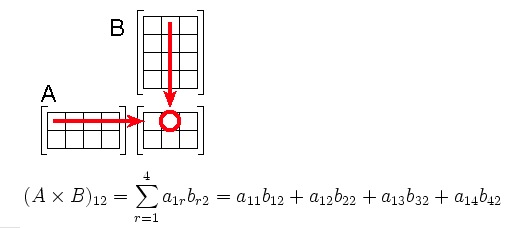
\includegraphics[width=8cm]{figures/matrixProduct.jpg}
\pause \\
\R{$\Q$} is a \B{column} vector. \R{$\P^T$} is a row vector.
%\R{$\P = \angles{ \P(1),\ldots,\P(n) }, \Q = \angles{ \Q(1),\ldots,\Q(m)}$}
\pause \\ ~\\
\R{$\M(\P,\Q) = \P^T \M \Q = \sum_{i=1}^n \sum_{j=1}^m \P(i) \M(i,j) \Q(j)$}
\end{frame}

\begin{frame}
  \frametitle{The minmax Theorem}
~\\
When using pure strategies, second player has an advantage.
~\\~\\ ~\pause
\B{John von Neumann, 1928.}
\\ ~ \\ 
\R{\[ \minp \maxq \mpq = \maxq \minp \mpq \]}
\\ ~ \\ 
In words: for \B{mixed} strategies, choosing second gives no advantage.
\end{frame}

\begin{frame}{The learning game matrix}
  \centering
  \begin{tabular}{lccc}
    \hline
    & \textbf{Example 1} & \textbf{Example 2} & \textbf{Example 3} \\
    \hline
    \textbf{Rule 1} & 0 & 1 & 0 \\
    \textbf{Rule 2} & 1 & 1 & 0 \\
    \textbf{Rule 3} & 0 & 0 & 1 \\
    \textbf{Rule 4} & 1 & 0 & 1 \\
    \textbf{Rule 5} & 0 & 1 & 1 \\
    \hline
  \end{tabular}
  ~\\~\\
  
  entries: 1 = rule is correct on example, 0= incorrect
\end{frame}

\begin{frame}
  \frametitle{Boosting is implied my min/max theorem}
  \begin{itemize}
  \item For any distribution \R{${\bf Q}$} over the examples there exists a row
    (rule) that is correct on \R{$\frac{1}{2} + \gamma$} of the (dist over the) examples.
  \item From min/max theorem we get that there exists a distribution \R{${\bf P}$} over the rules such that for any example at least\R{$\frac{1}{2} + \gamma$} of rhw (dist over the) rules are correct.
  \item The weighted majority is always correct.
  \item Existence proof, but not an algorithm.
  \end{itemize}
\end{frame}

\section{Schapire's algorithm}
\begin{frame}{Schapire's boosting algorithm}

  Calls the weak learner 3 times, on 3 different distributions, combines the rules using a majority.

  The distributions are
  \begin{itemize}
  \item \R{$h_1$}: use the training set as is.
  \item \R{$h_2$}: Filter examples so that \R{$P(h_1(x)=c(x))=\frac{1}{2}$}
    \item \R{$h_3$} Filter out examples such that \R{$h_1(x)=h_2(x)$}
  \end{itemize}
  
\end{frame}

\begin{frame}{Idea of proof}
  \begin{itemize}
  \item If errors of weak rules are at most $x<1/2$ then error of combined rule is at most \R{$3x^2-2x^3$}.
  \item   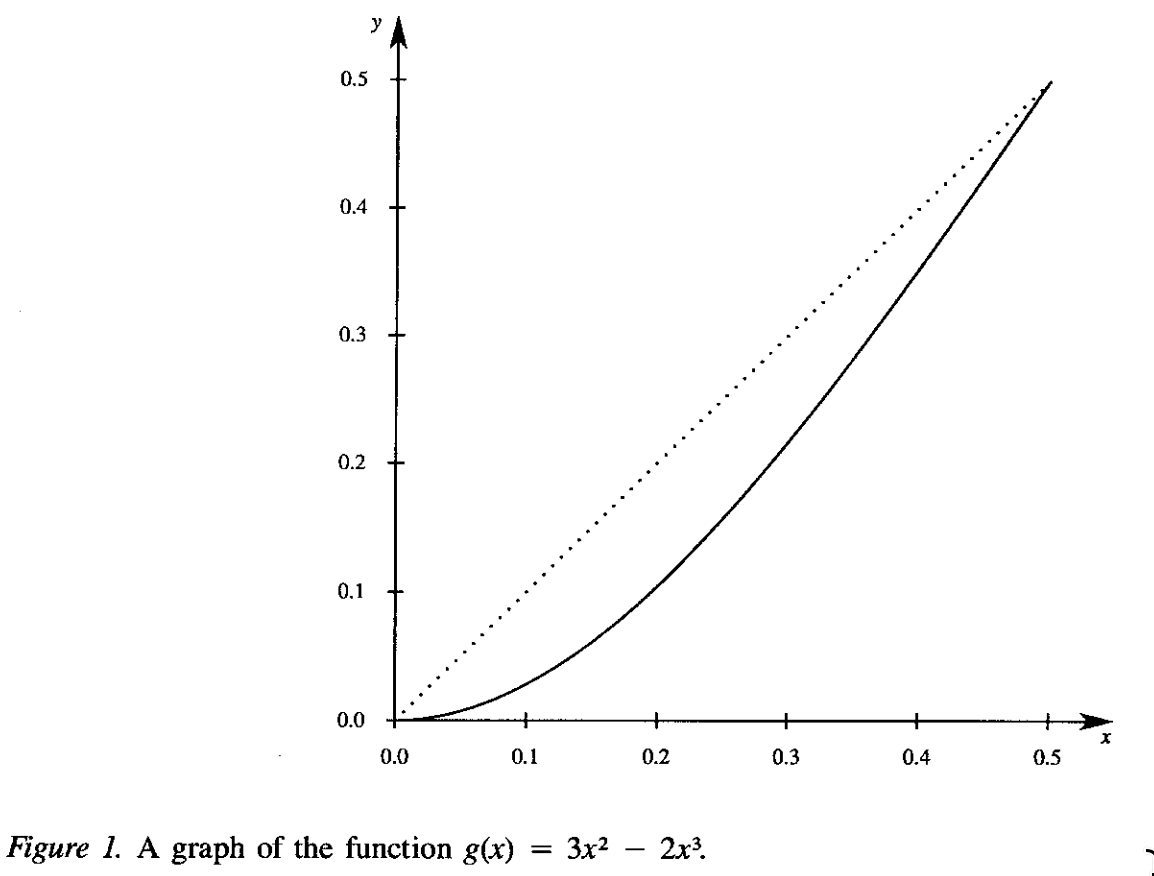
\includegraphics[width=5cm]{figures/SchapireBoostg-graph.png}
  \item Let the available rules have error $\frac{1}{2}-\gamma$ and assume we want a rule whose error is $\epsilon$.
  \item Using 3-combiner recursively for depth at most $O(\frac{1}{\gamma^2} \log \frac{1}{\epsilon})$
  achieves the error $\epsilon$.
  \end{itemize}
  \end{frame}

\section{Boost by Majority}
\begin{frame}{Boost By Majority}
  Majority vote over many weak rules, rather than 3.
  ~\\
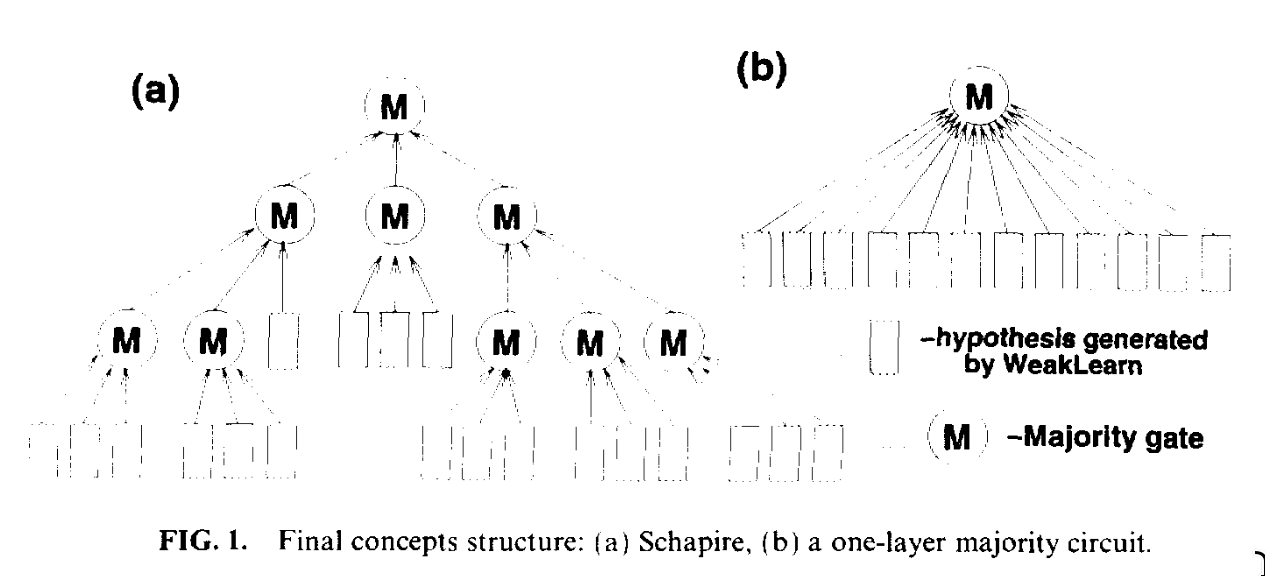
\includegraphics[width=8cm]{figures/BBMvsSchapire.png}
\end{frame}

\begin{frame}{Game between booster and learner}
  \begin{itemize}
  \item Booster chooses distribution over examples.
  \item Weak learner chooses where weak rules makes a mistake.
  \item Weak learner constrained to make weighted error smaller than \R{$(1/2)-\gamma$}
  \end{itemize}
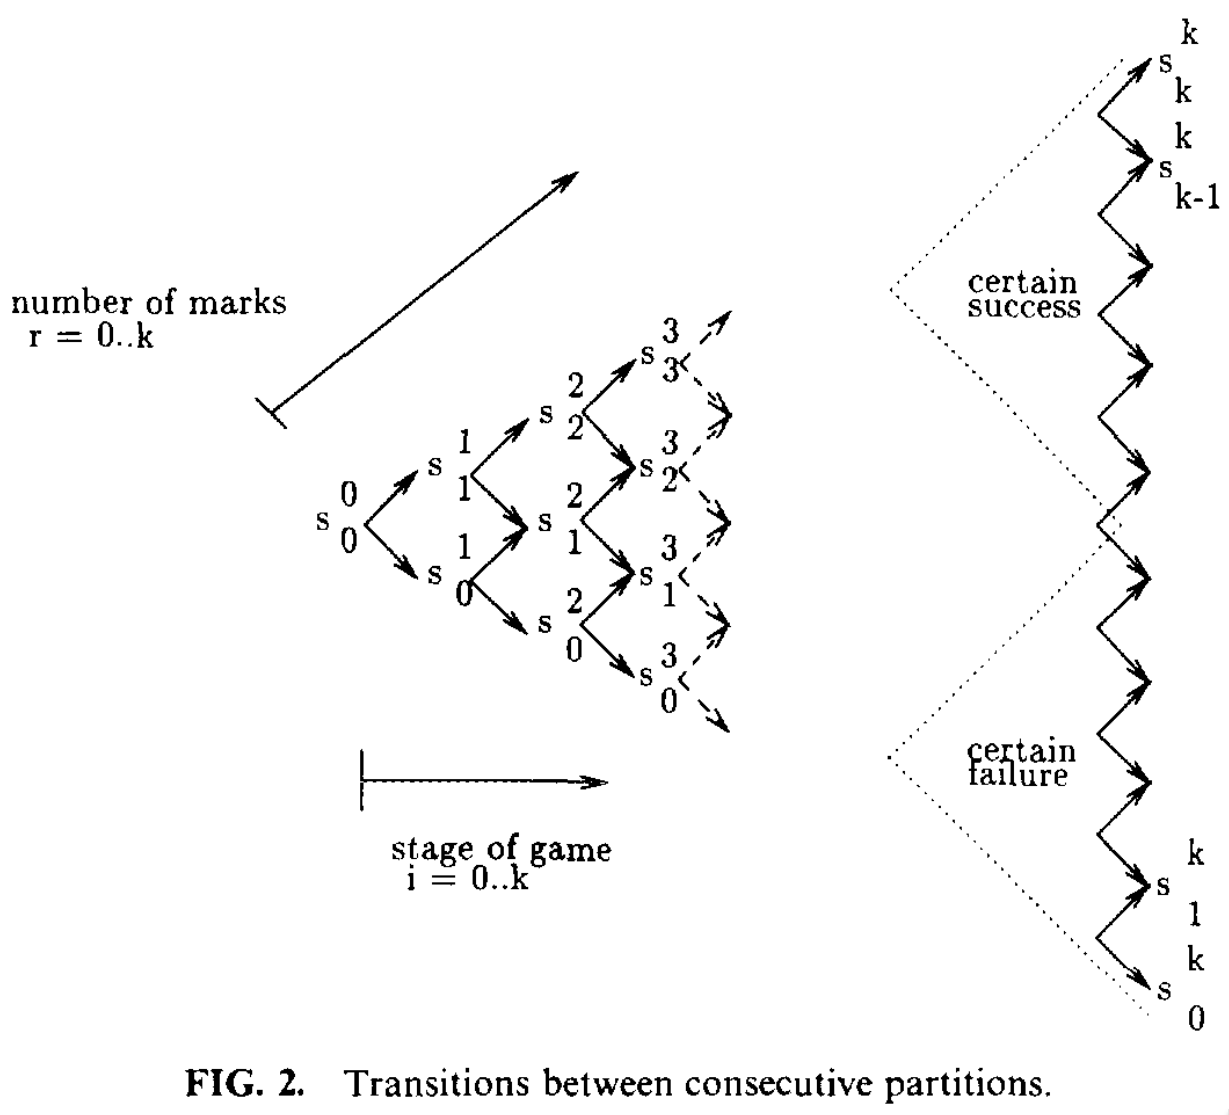
\includegraphics[width=6cm]{figures/BBMFigure.png}
\end{frame}

\begin{frame}{Potential function}
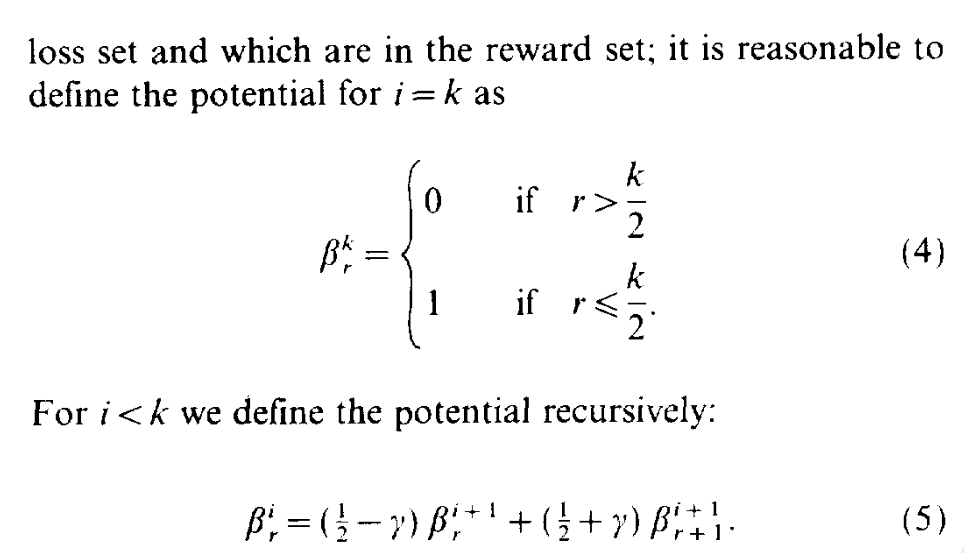
\includegraphics[width=8cm]{figures/BBMPotential.png}
\end{frame}

\begin{frame}{Weight function}
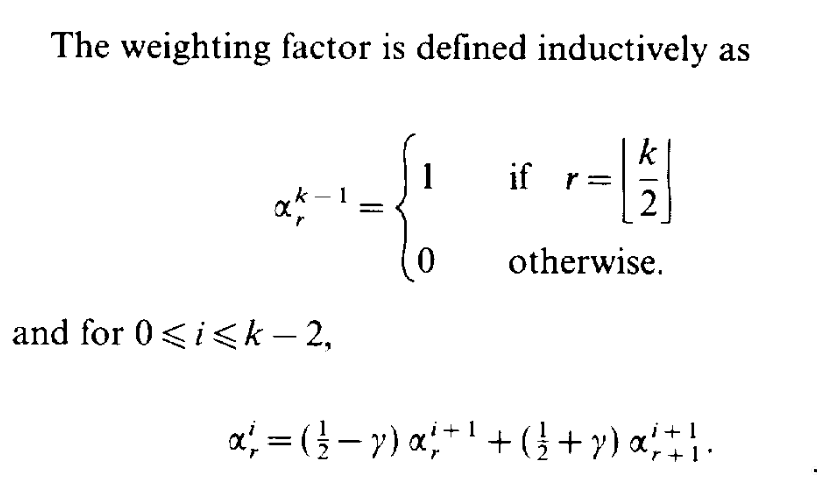
\includegraphics[width=8cm]{figures/BBMWeighting.png}
\end{frame}

\begin{frame}{Potential is non increasing}
  \begin{itemize}
  \item Let \R{$q_r^i$} be the fraction of the examples that have
    \R{$r$} mistakes on iteration \R{$i$}. 
  \item Then if the booster uses the weights $\alpha_r^i$ then
    \R{\[
        \beta_{0}^{0}
        \;>\;
        \sum_{r=0}^{1} q_{r}^{1}\,\beta_{r}^{1}
        \;>\;
        \sum_{r=0}^{2} q_{r}^{2}\,\beta_{r}^{2}
        \;>\;
        \cdots
        \;>\;
        \sum_{r=0}^{k} q_{r}^{k}\,\beta_{r}^{k}.
      \]}
    \item Idea of proof, consider last and next to last steps.
  \end{itemize}

\end{frame}

\begin{frame}{Error bound}

  Given a weak learner with error $(1/2)-\gamma$, find $k$ that satisfies
\R{\[
  \sum_{j=0}^{\left\lfloor \frac{k}{2} \right\rfloor}
  \binom{k}{j}
  \bigl(\tfrac12 + \gamma\bigr)^{j}\,
  \bigl(\tfrac12 - \gamma\bigr)^{\,k - j}
  \;\;\le\;\;
  \epsilon.
\]}
Then running Boost-by-majority for $k$ iterations will generate a rule with 
error at most $\epsilon$.

\end{frame}



\section{Adaboost}

\begin{frame}
  \frametitle{{Adaboost}}
\end{frame}
%------------------------------------------------
\begin{frame}{Algorithm AdaBoost (Setup)}
\textbf{Input:}
\begin{itemize}
  \item \R{Sequence of $N$ labeled examples $\langle (x_1,y_1),\ldots,(x_N,y_N)\rangle$}
  \item \R{Weak learning algorithm \textit{WeakLearn}}
  \item \R{Integer $T$ specifying number of iterations}
\end{itemize}

\textbf{Initialize:} 
\[
  \R{w_i^1 = \frac{1}{N}\quad \text{for } i=1,\ldots,N.}
\]
\end{frame}

%------------------------------------------------
\begin{frame}{Algorithm AdaBoost (Main Loop)}
\textbf{For} \R{$t = 1, 2, \ldots, T$:}
\begin{enumerate}
  \item \R{$p^t = \frac{w^t}{\sum_{i=1}^N w_i^t}\,.$}
  \item Call \R{\textit{WeakLearn}}, providing the distribution \R{$p^t$}. 
        Get back a hypothesis \R{$h_t : X \to \{0,1\}$}.
  \item Calculate the error of \R{$h_t$}: 
    \[
      \R{\epsilon_t = \sum_{i=1}^N p_i^t\,|\,h_t(x_i) - y_i\,|.}
    \]
  \item Set 
    \[
      \R{\beta_t = \frac{\epsilon_t}{1 - \epsilon_t}.}
    \]
  \item Update the weights:
    \[
      \R{w_i^{t+1} = w_i^t\,\beta_t^{\,\bigl(1 - |\,h_t(x_i)-y_i\,|\bigr)}.}
    \]
\end{enumerate}
\end{frame}

%------------------------------------------------
\begin{frame}{Algorithm AdaBoost (Final Output)}
\textbf{Output the final hypothesis} \R{$h_{final}$}, defined by:
\[
  \R{
    h_{final}(x) =
    \begin{cases}
      1, &\text{if } \sum_{t=1}^T \bigl(\ln \tfrac{1}{\beta_t}\bigr)\,h_t(x)
            \;\ge\; \tfrac12 \sum_{t=1}^T \ln \tfrac{1}{\beta_t},\\[6pt]
      0, &\text{otherwise}.
    \end{cases}
  }
\]
\end{frame}


% --- Theorem Slide ---
\begin{frame}{Main Theorem}
  \textbf{Theorem 6} 
  Suppose the weak learning algorithm \R{\text{WeakLearn}}, 
  when called by \R{\text{AdaBoost}}, 
  generates hypotheses with errors \R{$\epsilon_1, \ldots, \epsilon_T$}. 
  Then the error 
  \R{$\epsilon = \frac{1}{N} \#[h_{final}(x_i) \neq y_i]$} 
  of the final hypothesis \R{$h_{final}$} is bounded above by
  \[
    \R{\epsilon \;\le\; 2^T \prod_{t=1}^T \sqrt{\epsilon_t \,\bigl(1 - \epsilon_t\bigr)}.}
  \]
\end{frame}

% --- Proof Slide ---
\begin{frame}{Upper bound on total weight}
  
  \R{
    \begin{eqnarray*}
    \sum_{i=1}^N w_i^{t+1}
      &\;=\;& \sum_{i=1}^N w_i^t \,\beta_t^{\,\bigl(1 - |\,h_t(x_i) - y_i\,|\bigr)} \\
      &\;\le\;& \sum_{i=1}^N w_i^\prime 
      \Bigl(1 - (1-\beta_t)\bigl(1 - |\,h_t(x_i) - y_i\,|\bigr)\Bigr)\\
      & \;\le\;& \Bigl(\sum_{i=1}^N w_i^t\Bigr)\!
               \Bigl(1 - (1-\epsilon_t)\,\bigl(1 - \beta_t\bigr)\Bigr).
    \end{eqnarray*}
    }
\end{frame}

%------------------------------------------------
\begin{frame}{Combining over iterations}
Combining the weight‐update inequality over \R{$t = 1,\ldots,T$}, we get 
\[
  \R{\sum_{i=1}^N w_i^{T+1} 
       \le \prod_{t=1}^T 
         \Bigl(1 - (1-\epsilon_t)\,(1-\beta_t)\Bigr).}
  \tag{16}
\]
\end{frame}

\begin{frame}{Lower bound on total weight}
The final hypothesis \R{$h_{final}$} makes a mistake on instance \R{$i$} only if
\[
  \R{
    \prod_{t=1}^T \beta_t^{\,\bigl(1-|\,h_t(x_i)-y_i\,|\bigr)}
    \;\ge\;
    \Bigl(\prod_{t=1}^T \beta_t\Bigr)^{-\tfrac12}.
  }
  \tag{17}
\]

The final weight of instance \R{$i$} is
\[
  \R{w_i^{T+1} = D(i)\,\prod_{t=1}^T \beta_t^{\,\bigl(1-|\,h_t(x_i)-y_i\,|\bigr)}.}
  \tag{18}
\]

By comparing the sum of all final weights to those on examples where \R{$h_{final}$} is incorrect, one obtains
\[
  \R{\sum_{i=1}^N w_i^{T+1}
       \;\ge\;
       \sum_{\,i : h_{final}(x_i)\neq y_i\,} w_i^{T+1}
       \;\ge\;
       e \,\Bigl(\prod_{t=1}^T \beta_t\Bigr)^{\!1/2},}
\]
where \R{$e$} is the error of \R{$h_{final}$}. 
\end{frame}

%------------------------------------------------
\begin{frame}{Resulting Error Bound}
Combining (16) and the above,
\[
  \R{
    e 
    \;\le\;
    \prod_{t=1}^T \frac{\,1 - (1-\epsilon_t)\,(1-\beta_t)\,}{\sqrt{\beta_t}}.
  }
  \tag{20}
\]
Minimizing each factor leads to \R{$\beta_t = \epsilon_t / (1-\epsilon_t)$}. Plugging back yields
\[
  \R{
    e 
    \;\le\;
    2^T \,\prod_{t=1}^T \sqrt{\epsilon_t\,(1-\epsilon_t)},
  }
\]
\end{frame}

\begin{frame}{Alternative forms of the bound}
  \R{
    \begin{eqnarray*}
      e &\;\le\;& \prod_{t=1}^T \sqrt{\,1 - 4\,\gamma_t^2}
      \;=\; \exp\Bigl(-\sum_{t=1}^T \mathrm{KL}\bigl(\tfrac12\,\|\,\tfrac12 - \gamma_t\bigr)\Bigr)\\
      &\;\le\;&
      \exp\Bigl(-2\sum_{t=1}^T \gamma_t^2\Bigr).
    \end{eqnarray*}
  }
\end{frame}



\begin{frame}{Comparing Hedge vs Adaboost}
  \begin{columns}[T,onlytextwidth] 
    % [T] aligns columns at the top; [onlytextwidth] allows full use of slide width.

    \column{0.48\textwidth}
    \textbf{Hedge}
    \begin{itemize}
      \item Each iteration adds an Example
      \item Weights assigned to Experts
      \item Upper bound on potential: Loss of alg.
      \item Lower bound on potential: Loss of best expert
    \end{itemize}

    \column{0.48\textwidth}
    \textbf{Adaboost}
    \begin{itemize}
    \item Each iteration adds a Weak Rule
    \item Weights assigned to examples.
    \item Upper bound on Potential: Edges of weak rules.
    \item Lower bound on Potential: Error of majority vote.
    \end{itemize}

  \end{columns}
\end{frame}

\begin{frame}{Main Concepts}
  \begin{itemize}
    \item \B{Margin:} the coordinate of interrest \R{$x$}
  \item \B{Potential:} An upper bound on the error. \R{$\phi(x)$}
  \item \B{Weight:} The gradient of the potential. \R{$\nu = \frac{\partial}{\partial x} \phi(x)$}
  \end{itemize}

  
  \end{frame}

\end{document}

\section{Repeated Matrix Games}

\begin{frame}
\frametitle{Zero sum games in matrix form}
\begin{itemize}
\item Game between two players.
\item Defined by \R{$n \times m$} matrix \R{$\M$}
\item \B{Row} player chooses \R{$i \in \{1,\ldots,n\}$}
\item \B{Column} player chooses \R{$j \in \{1,\ldots,m\}$}
\item \B{Row} player gains \R{$\M(i,j) \in [0,1]$}
\item \B{Column} player looses \R{$\M(i,j)$}
\item Game repeated many times.
\end{itemize}
\end{frame}

\begin{frame}
\frametitle{Pure vs. mixed strategies}
\begin{itemize}
\item Choosing a \B{single} action = \B{pure} strategy.
\item Choosing a \B{Distribution} over actions = \B{mixed} strategy.
\item \B{Row} player chooses dist. over rows \R{$\P$}
\item \B{Column} player chooses dist. over columns \R{$\Q$}
\item \B{Row} player gains \R{$\M(\P,\Q)$}.
\item \B{Column} player looses \R{$\M(\P,\Q)$}.
\end{itemize}
\end{frame}

\begin{frame}
\frametitle{Mixed strategies in matrix notation}
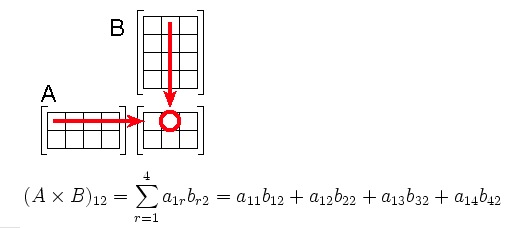
\includegraphics[width=8cm]{figures/matrixProduct.jpg}
\pause \\
\R{$\Q$} is a \B{column} vector. \R{$\P^T$} is a row vector.
%\R{$\P = \angles{ \P(1),\ldots,\P(n) }, \Q = \angles{ \Q(1),\ldots,\Q(m)}$}
\pause \\ ~\\
\R{$\M(\P,\Q) = \P^T \M \Q = \sum_{i=1}^n \sum_{j=1}^m \P(i) \M(i,j) \Q(j)$}
\end{frame}

\begin{frame}
  \frametitle{The minmax Theorem}
~\\
When using pure strategies, second player has an advantage.
~\\~\\ ~\pause
\B{John von Neumann, 1928.}
\\ ~ \\ 
\R{\[ \minp \maxq \mpq = \maxq \minp \mpq \]}
\\ ~ \\ 
In words: for \B{mixed} strategies, choosing second gives no advantage.
\end{frame}


\begin{frame}
\frametitle{Minmax is weaker than diminishing regret}
\begin{itemize}
\item The minmax theorem proves the existence of an \B{Equilibrium}.
\item Learning guarantees no regret with respect to the past.
\item If all sides use learning, then game will converge to minmax equilibrium.
\item If opponent is not optimally adversarial (limited by knowledge, computationa power...) then learning gives \B{better} performance than min-max.
\item Our goal is to minimize regret.
\end{itemize}
\end{frame}


%%% Local Variables:
%%% mode: latex
%%% TeX-master: t
%%% End:
